% Author: Dr. Matthias Jung, DL9MJ
% Year: 2022
\documentclass[convert=false]{standalone}
\input{../common/settings.tex}
\usepackage{tikz,pgfplots}
\usepgfplotslibrary{fillbetween}

\begin{document} 
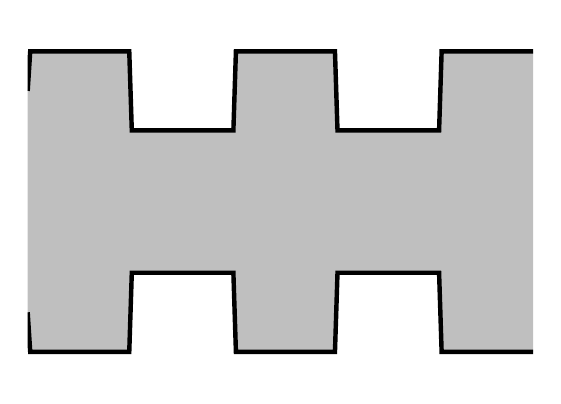
\begin{tikzpicture}
    \pgfplotsset{samples=200}
    \begin{axis}[
        width=8cm,
        height=6cm,
        axis lines=none,
        ticks=none,
        xmin =  0,
        ymin = -2.2,
        xmax =  8.8,
        ymax =  2.2,
        domain = 0:8.8,
        thick,
        no markers]
        \addplot+[name path=A,ultra thick, black] { 0.5*sign(sin(deg(x*1.75)))+1.4};
        \addplot+[name path=B,ultra thick, black] {-0.5*sign(sin(deg(x*1.75)))-1.4};
        \addplot[gray, opacity=0.5] fill between[of=A and B];
    \end{axis}
\end{tikzpicture}
\end{document}